In this Section we study the power of the center of the system over several classic concentric, axis-aligned Poncelet families. A key observation is that said power remains constant with respect to two classic circles (the circumcircle and Euler's circle), despite the fact that their centers and radii variable.

\subsection{Pair with Incircle}

Consider an ellipse pair where the inner ellipse is a circle of radius $r$; see Figure~\ref{fig:incircle}. The Cayley condition for 3-periodics reduces to $r=(a b)/(a+b)$ \cite[Coroll. 1]{garcia2020-family-ties}. By definition, the incenter $X_1$ lies at the origin and the inradius is constant.

Remarkable properties of this family include the fact that (i) it conserves the sum of cosines, (ii) the circumradius $R$ is invariant, and (iii) the locus of both $X_3$ and $X_5$ are circles\footnote{Amongst the first 201 centers in \cite{etc} the loci of the following are circles concentric with $X_1$: $X_k$, $k=$3, 5, 11, 12, 35, 36, 40, 46, 55, 56, 57, 65, 80, 119, 165 \cite{garcia2020-family-ties}.} concentric with $X_1$. Let $r_3$ and $r_5$ denote their radii, respectively. These are given by \cite[Section 3]{garcia2020-family-ties}:

\[ R = \frac{a+b}{2},\;\;\;r_3 = \frac{a-b}{2},\;\;\;r_5 = \frac{(a-b)^2}{4(a+b)}\]

\begin{proposition}
Over 3-periodics in the concentric pair with incircle, the power of the center $O=X_1$ with respect to either circumcircle \cite[Prop. 1]{garcia2020-family-ties} and Euler's circle are invariant and given by:

\[ \P_3= -a b,\;\;\;\P_5= -a b \frac{a^2 + b^2}{2(a + b)^2}\]

\end{proposition}

\begin{proof}
We compute powers wrt circumcircle and Euler circle as functions of sidelengths $s_1,s_2,s_3$:

\[ \P_3 = -\frac{s_1 s_2 s_3}{s_1 + s_2 + s_3} \]

\[\P_5 = \frac{-(s_1^3 + s_2^3 + s_3^3 - s_1^2(s_2 + s_3) - s_2^2(s_3 + s_1) - s_3^2(s_1 + s_2) + 4 s_1 s_2 s_3 )}{4 (s_1 + s_2 + s_3)} \]

$\P_3$ is $-1/{\pi}$ times the area of the circumellipse centered on the incenter, i.e., $\P_3 = -a b$. In order to simplify $\P_5$ formula we derive the following parametrization for the sidelengths:

\[ s_1 = \frac{w \tau}{r},\;\;\;
 s_2 = \frac{4r(r^2 + (1 - t)w)}{(2r^2 + (1 - t)w)\tau + (1 - t)z},\;\;\;
 s_3 = \frac{4r(r^2 + (1 - t)w)}{(2r^2 + (1 - t)w)\tau - (1 - t)z}\]

\noindent with $\tau=\sqrt{1-t^2}$ and $z =\sqrt{4r^2(t - 1)w + (1 - t^2)w^2 - 4r^4}$, $r =(ab)/(a + b)$, and $w = ab$. Replacing $s_1$, $s_2$, $s_3$ obtain $\P_5 = r^2 - 1/2 w$ and the formula in the proposition.
\end{proof}

\begin{figure}
    \centering
    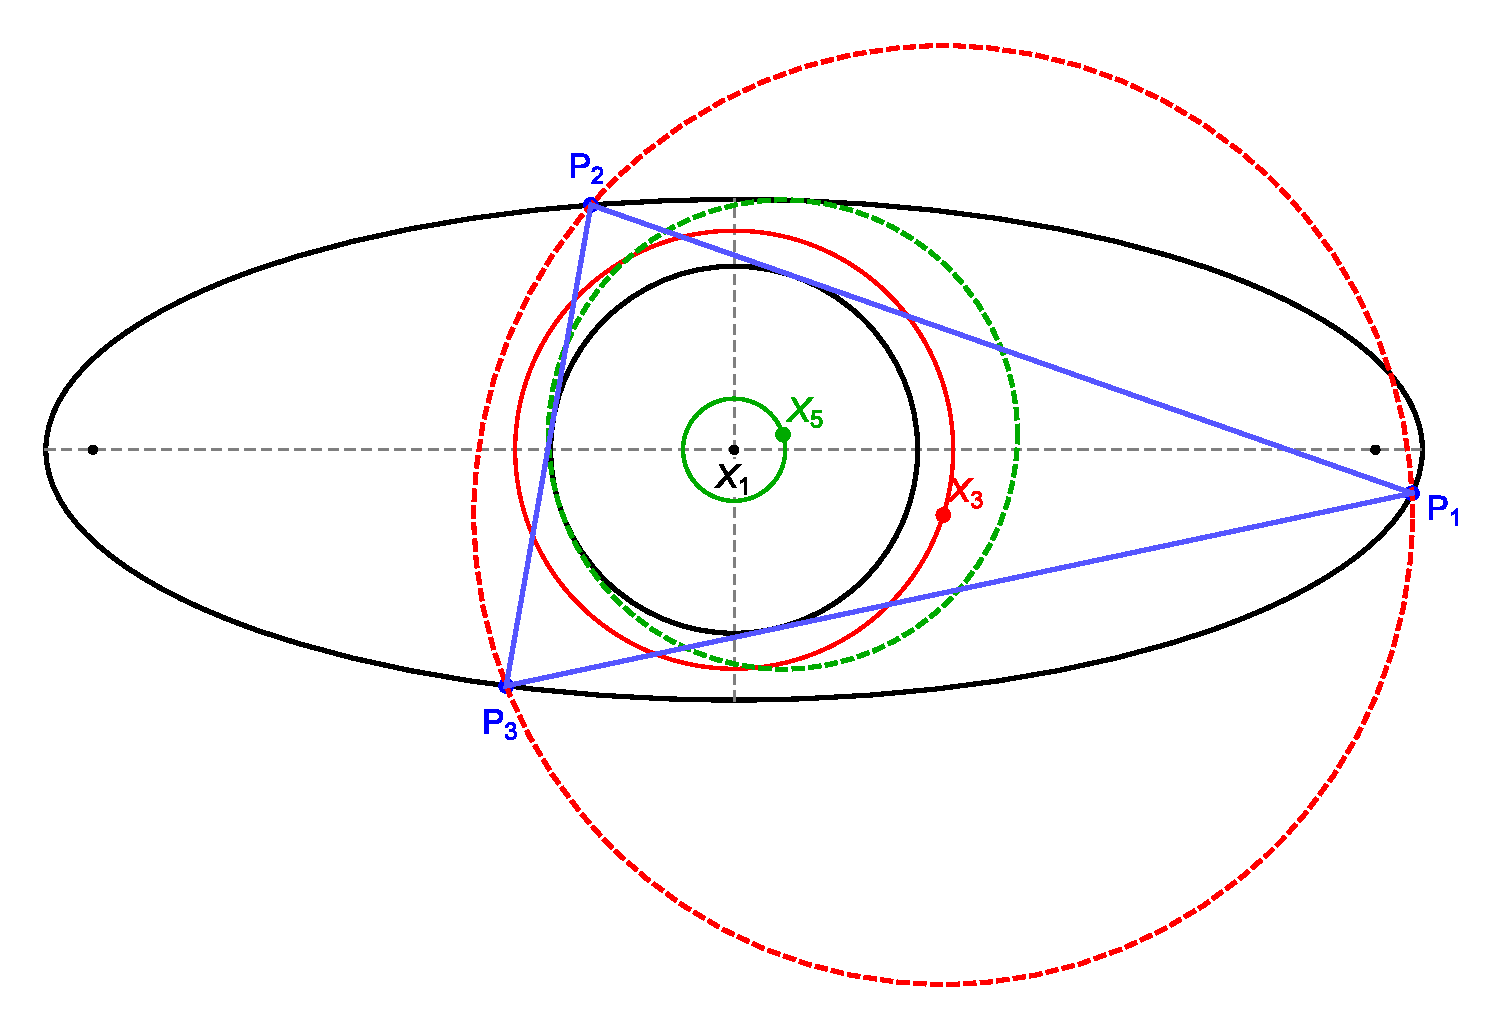
\includegraphics[width=.7\textwidth]{pics/0040_n3_incircle.eps}
    \caption{In the ellipse pair with incircle, the locus of both $X_3$ and $X_5$ are concentric circles (red and green). The power of the center $O=X_1$ wrt to either the circumcircle (dashed red) or Euler's circle (dashed green) is invariant. \href{https://bit.ly/3snkrJc}{live}}
    \label{fig:incircle}
\end{figure}

\subsection{Pair with Circumcircle}

Consider an ellipse pair where the outer ellipse is a circle of radius $a=b=R$ and the inner one is a concentric ellipse  with semi-axes $(a_c,b_c)$. The Cayley condition for 3-periodics to exist reduces to $a_c+b_c=R$ \cite{garcia2020-family-ties}. By definition, the incenter $X_3$ lies at the origin and the circumradius $R$ is constant. Invariants known to this family include the product of cosines and the sum of sidelengths squared \cite{garcia2020-family-ties}. Referring to Figure~\ref{fig:circumcircle}:

\begin{proposition}
Over 3-periodics in the concentric pair with circumcircle, the locus of $X_5$ is a circle\footnote{Amongst the first 201 centers in \cite{etc} the loci of the following are circles concentric with $X_3$: $X_k$, $k=$2, 4, 5, 20, 22, 23, 24, 25, 26, 74, 98, 99, 100, 101, 102, 103, 104, 105, 106, 107, 108, 109, 110, 111, 112, 140, 156, 186, 201 \cite{garcia2020-family-ties}.} concentric with original pair whose radius $r_5$ is given by $r_5= ({a_c-b_c})/{2}$. 
\end{proposition}

\begin{figure}
    \centering
    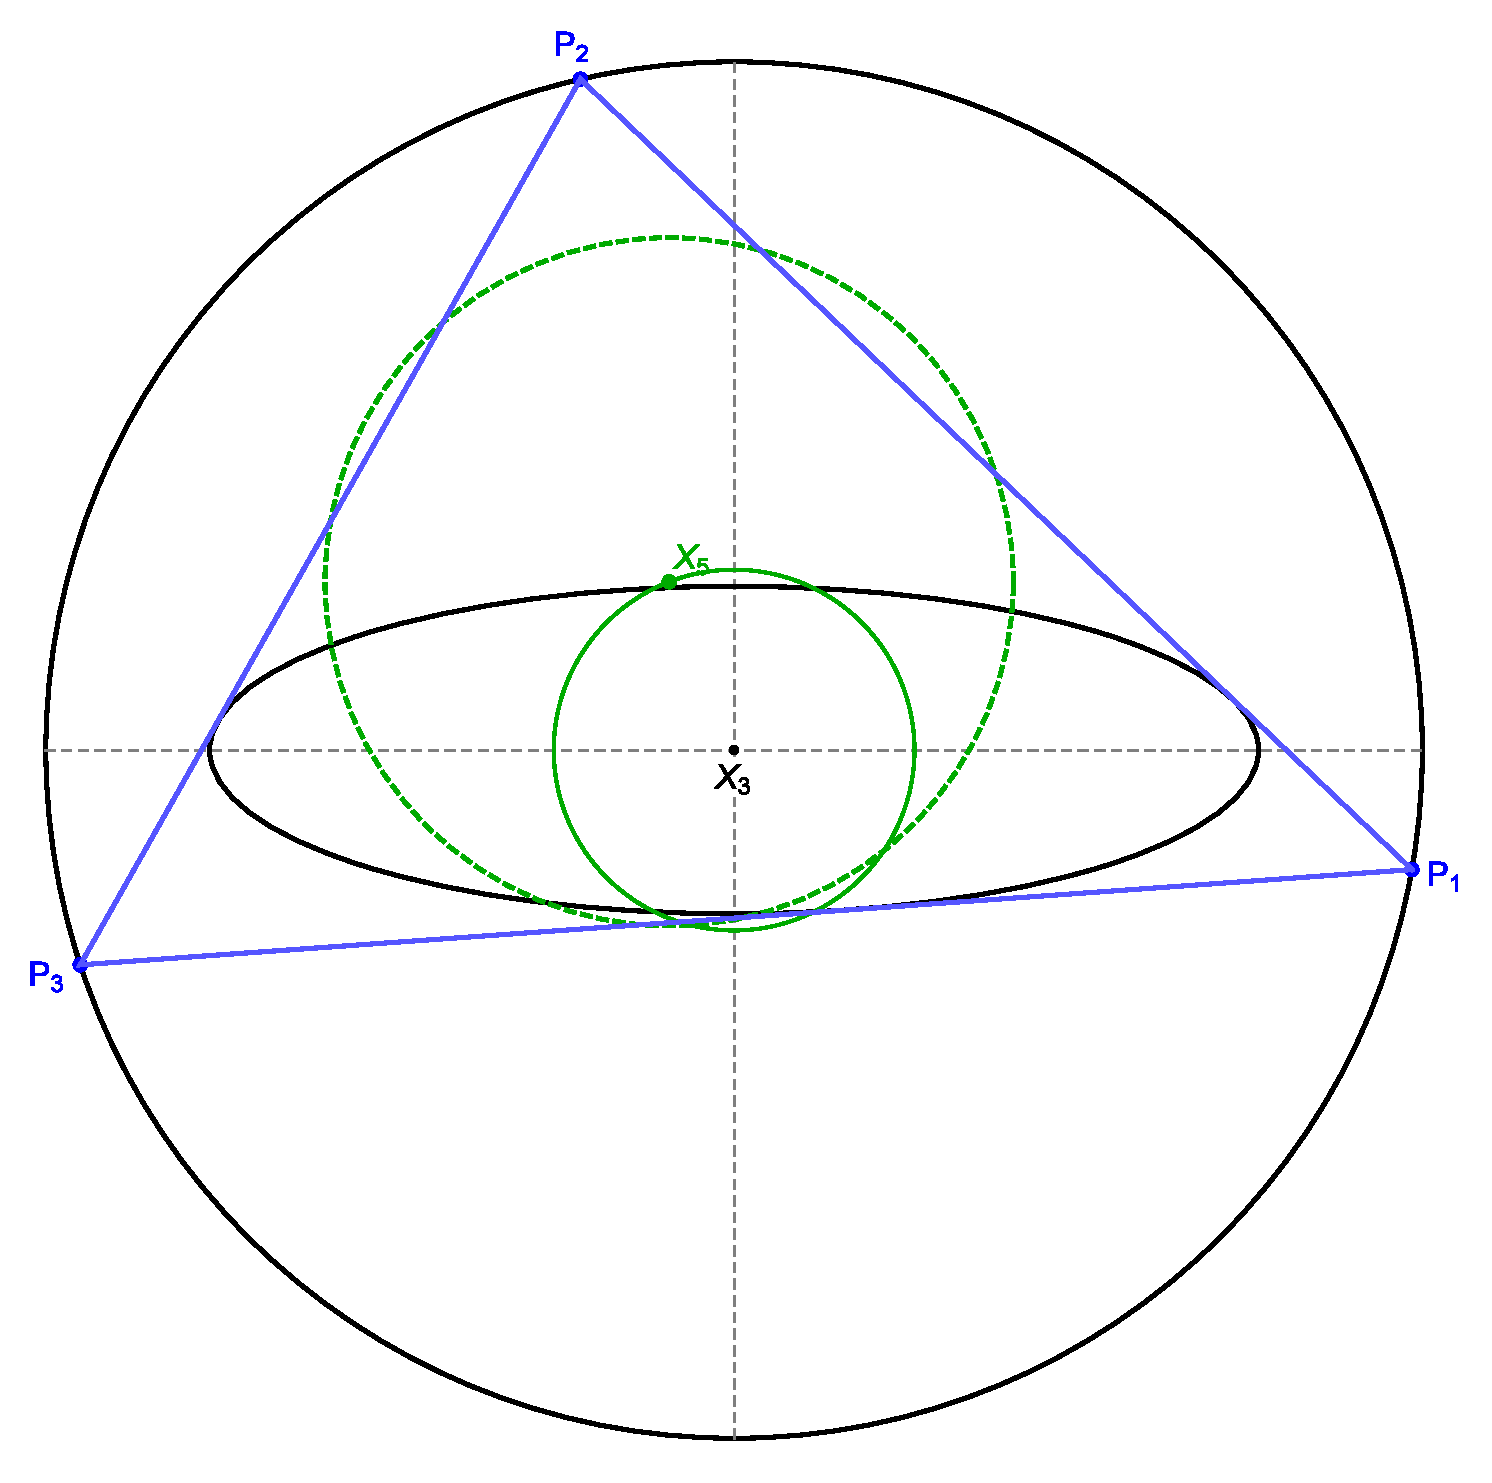
\includegraphics[width=.5\textwidth]{pics/0060_n3_circumcircle.eps}
    \caption{A circle and a concentric inellipse and a  3-periodic (blue). By definition, $X_3$ is stationary at the common center and the circumradius $R$ is constant. The locus of the center $X_5$ of Euler's circle (dashed green) is a concentric circle (solid green). \href{https://bit.ly/31nIg84}{live}}
    \label{fig:circumcircle}
\end{figure}

\begin{corollary}
Over 3-periodics in the concentric pair with circumcircle, the power of the center $O=X_3$ with respect to either circumcircle or Euler's circle is invariant and given by:

\[ \P_3 = -R^2,\;\;\;\P_5 = r_5^2-(R/2)^2 = -a_c b_c\]
\end{corollary}


\subsection{Homothetic Pair}

Consider a pair of concentric, homothetic ellipses admitting a 3-periodic family (elliptic billiard); see Figure~\ref{fig:homothetic}.


\begin{figure}
    \centering
    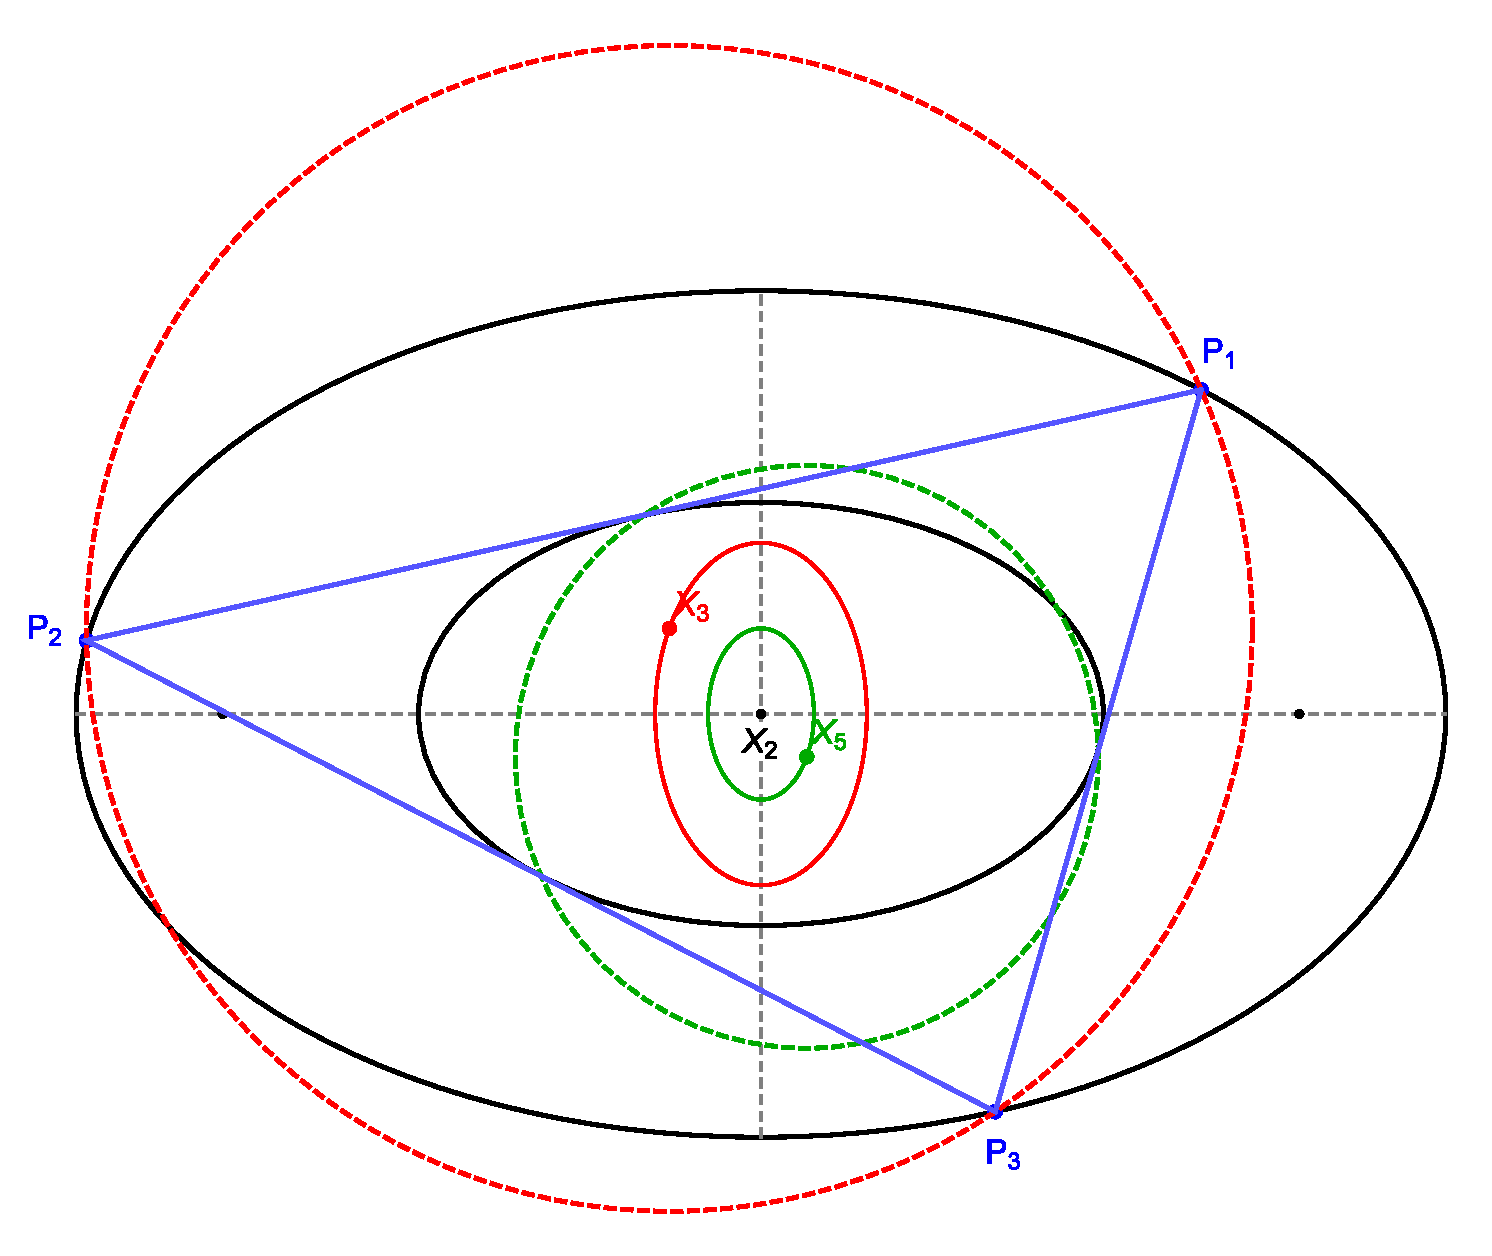
\includegraphics[width=.7\textwidth]{pics/0130_n3_homothetic.eps}
    \caption{A concentric, homothetic pair of ellipses (black) and a 3-periodic (blue) interscribed between them. The barycenter $X_2$ is stationary at the common center. Over the family, the locus of $X_3$ and $X_5$ are concentric ellipses (solid red and green). The power of the center wrt the circumcircle (dashed red) and Euler's circle (dashed green) is invariant. \href{https://bit.ly/3vZEr6W}{live}}
    \label{fig:homothetic}
\end{figure}

This family conserves area and sum of squared sidelengths, and consequently the Brocard angle \cite{reznik2020-similarityII}. The Barycenter $X_2$ is stationary at $O$. The Cayley condition implies that $(a_c,b_c)=(a/2,b/2)$.

Over this family, the locus of both $X_3$ and $X_5$ are ellipses concentric and axis-aligned with the original pair \cite{garcia2020-family-ties}. Their semi-axes are given by:

\[(a_3,b_3)=\frac{c^2}{4}\left(\frac{1}{a},\frac{1}{b}\right),\;\;\text{and}\;\;
	(a_5,b_5)=\frac{c^2}{8}\left(\frac{1}{a},\frac{1}{b}\right) \]

%\[ A=\frac{3\sqrt{3}ab}{2}, \;\;\;\;\; \sum{s_i}^2=\frac{9}{2}(a^2+b^2)\cdot\]

\noindent Nevertheless:

\begin{proposition}
Over 3-periodics in the homothetic pair, the power of the center $O=X_2$ with respect to both the circumcircle and Euler circle are invariant and given by:

\[ 
\P_3 = -\frac{a^2+b^2}{2},\;\;\;\P_5=-\frac{a^2+b^2}{8} \]
\end{proposition} 

\begin{proof}
Squared radii and squared distances between barycenter $X_2$ and circumcenter $X_3$ or nine-point center $X_5$ can be obtained via direct computation and in terms of squared sidelengths. This yields:

\[
\P_3 = -\frac{1}{9}\ \sum{ s_i^2},\;\;\;
\P_5= -\frac{1}{36}\sum{s_i^2} \]

Recall the sum of squared sidelengths is conserved in the homothetic pair and given by \cite[Remark 2.1]{reznik2020-similarityII}:

\[  \sum{s_i}^2=\frac{9}{2}(a^2+b^2)\]

\end{proof}

\subsection{Confocal Pair}

Consider a confocal pair of ellipses which admits a 3-periodic family (elliptic billiard); see Figure~\ref{fig:confocal}. Classic invariants include perimeter and Joachmisthal's constant \cite{sergei91}. A recent result is that the sum of angle cosines is invariant \cite{reznik2020-intelligencer,garcia2020-new-properties}. The Mittenpunkt $X_9$ is stationary at $O$ \cite{reznik2020-intelligencer}. The semi-axes of the inner ellipse are given by \cite{garcia2019-incenter}:

\begin{equation}
[a_c,b_c] = \frac{1}{c^2}\left[a(\delta-b^2),\;b(a^2-\delta)\right]
\label{eqn:confocal-axes}
\end{equation} 

\noindent where $\delta^2={a^4-a^2 b^2+b^4}$.

Furthermore, over said family, the locus of both $X_3$ and $X_5$ are concentric, axis-aligned ellipses with semi-axes are given by \cite{garcia2020-ellipses}:

\begin{align*}
    [a_3,b_3]=&\left[\frac{a^2-\delta}{2a},\frac{\delta-b^2}{2b}\right]\\
%    [a_5,b_5]=&\left[\frac{- w'_5(a,b)+ w''_5(a,b) \delta}{ w_5(a,b)},\;\frac{ w'_5(b,a)-{w''_5(b,a) \delta}}{w_5(b,a)}\right] \\
    [a_5,b_5]=&\left[\frac{- w_2(a,b)+ w_3(a,b) \delta}{ w_1(a,b)},\;\frac{ w_2(b,a)-{w_3(b,a) \delta}}{w_1(b,a)}\right]
\end{align*}

\noindent where $w_1(u,v)=4u(u^2-v^2)$, $w_2(u,v)=u^2(u^2+3v^2)$, $w_3(u,v)=3u^2+ v^2$.

Recall that over 3-periodics in the confocal pair, $\P_3=-\delta$ \cite[Thm. 3]{garcia2020-new-properties}. We extend this to $\P_5$:

\begin{proposition}
 Over 3-periodics in the confocal pair, the power of the center $O=X_9$ with respect to Euler's circle is invariant and given by:

% \[ \P_3 = \frac{-(3 + h^2)((3 + h) a^2 + (3 - h) b^2)}{2(9 - h^2)} = -\delta \]

% \[ \P_5 =& \frac{-(3 - h^2)(1 - h^2)((3 + h) a^2 + (3 - h) b^2)}{8(9 - h^2)} = -\eta \]

%\[ \P_5 =  -\frac{\delta(a^4+b^4+\delta)}{c^4} \]

\[ \P_5 =  \frac{\delta \mu \eta (\mu^2 + \eta^2 - 2 )}{\mu^2 + \eta^2 + 1} \]

\noindent where $\mu= {a}/{a_c}$ and $\eta= {b}/{b_c}$.
\end{proposition}

\begin{proof}

Straightforward computation of power of $O=X_9$ with respect to circumcircle and Euler circle gives:

\[P_3 = \frac{ -(s_1^3 + s_2^3 + s_3^3 - s_1^2 (s_2 + s_3) - s_2^2 (s_3 + s_1)  - s_3^2 (s_2 + s_1) + 6 s_1 s_2 s_3) s_1 s_2 s_3 }{(s_1^2 + s_2^2 + s_3^2 - 2 s_1 s_2 - 2 s_2 s_3 - 2 s_3 s_1)^2 }\]

\[\P_5 = \kappa \frac{ (s_1^3 + s_2^3 + s_3^3 - s_1^2 (s_2 + s_3) - s_2^2 (s_3 + s_1)  - s_3^2 (s_2 + s_1))}{(s_1^2 + s_2^2 + s_3^2 - 2 s_1 s_2 - 2 s_2 s_3 - 2 s_3 s_1)^2 } \]

\noindent where $\kappa=(s_1 + s_2 - s_3)(s_1 - s_2 + s_3)(-s_1 + s_2 + s_3)$.

We use the following parametrization for 3-periodics $P_1P_2P_3$ in the confocal pair. Let $\rho$ denote the invariant $r/R$ ratio (inradius/circumradius), $s$ the invariant semi-perimeter, and $c_1$ the cosine of the internal angle at $P_1$:

\[ s_1 = \frac{2(1 - c_1) s}{\rho - 2 c_1 + 2},\;\;\;s_2 = \frac{(\rho c_1 - c_1^2 + \rho + 1 - w) s}{(1 + c_1)(\rho - 2 c_1 + 2)},\;\;\;s_3 = \frac{(\rho c_1 - c_1^2 + \rho + 1 + w) s}{(1 + c_1)(\rho - 2 c_1 + 2)}\]

\noindent where $h^2=1-2\rho$, and $w^2 = (1 - c_1^2) (h^2 - (c_1 - \rho)^2)$. The squared semi-axis lengths are given by: 

\[ a^2 = \frac{4(1 + h)s^2}{(3 - h)(3 + h)^2},\;\;\;b^2 = \frac{4(1 - h)s^2}{(3 + h)(3 - h)^2} \]

\noindent Substituting $s_1$, $s_2$, $s_3$ in $\P_3$ and $\P_5$ we get powers with respect to the circles:

\[ \P_3 = \frac{-4(3 + h^2) s^2}{(9 - h^2)^2},\;\;\;
\P_5 = \frac{-(3 - h^2)(1 - h^2)s^2}{(9 - h^2)^2} \]


which doesn't depend of variable parameter $c_1$.

These values are always negative since $O$ is interior to both the circumcircle and Euler circle.

Finally, using $a_c/a = (1 + h)/2$ and $b_c/b = (1 - h)/2$ we get the formulas in the proposition.

%\textcolor{red}{from dominique to dan : notice that \[ h = a_c/a - b_c/b \] so now we have a beautiful formula for $\rho$ ratio inradius/circumradius \[ \rho = (1 - (a_c/a - b_c/b)^2)/2 \]}

\end{proof}

\begin{figure}
    \centering
    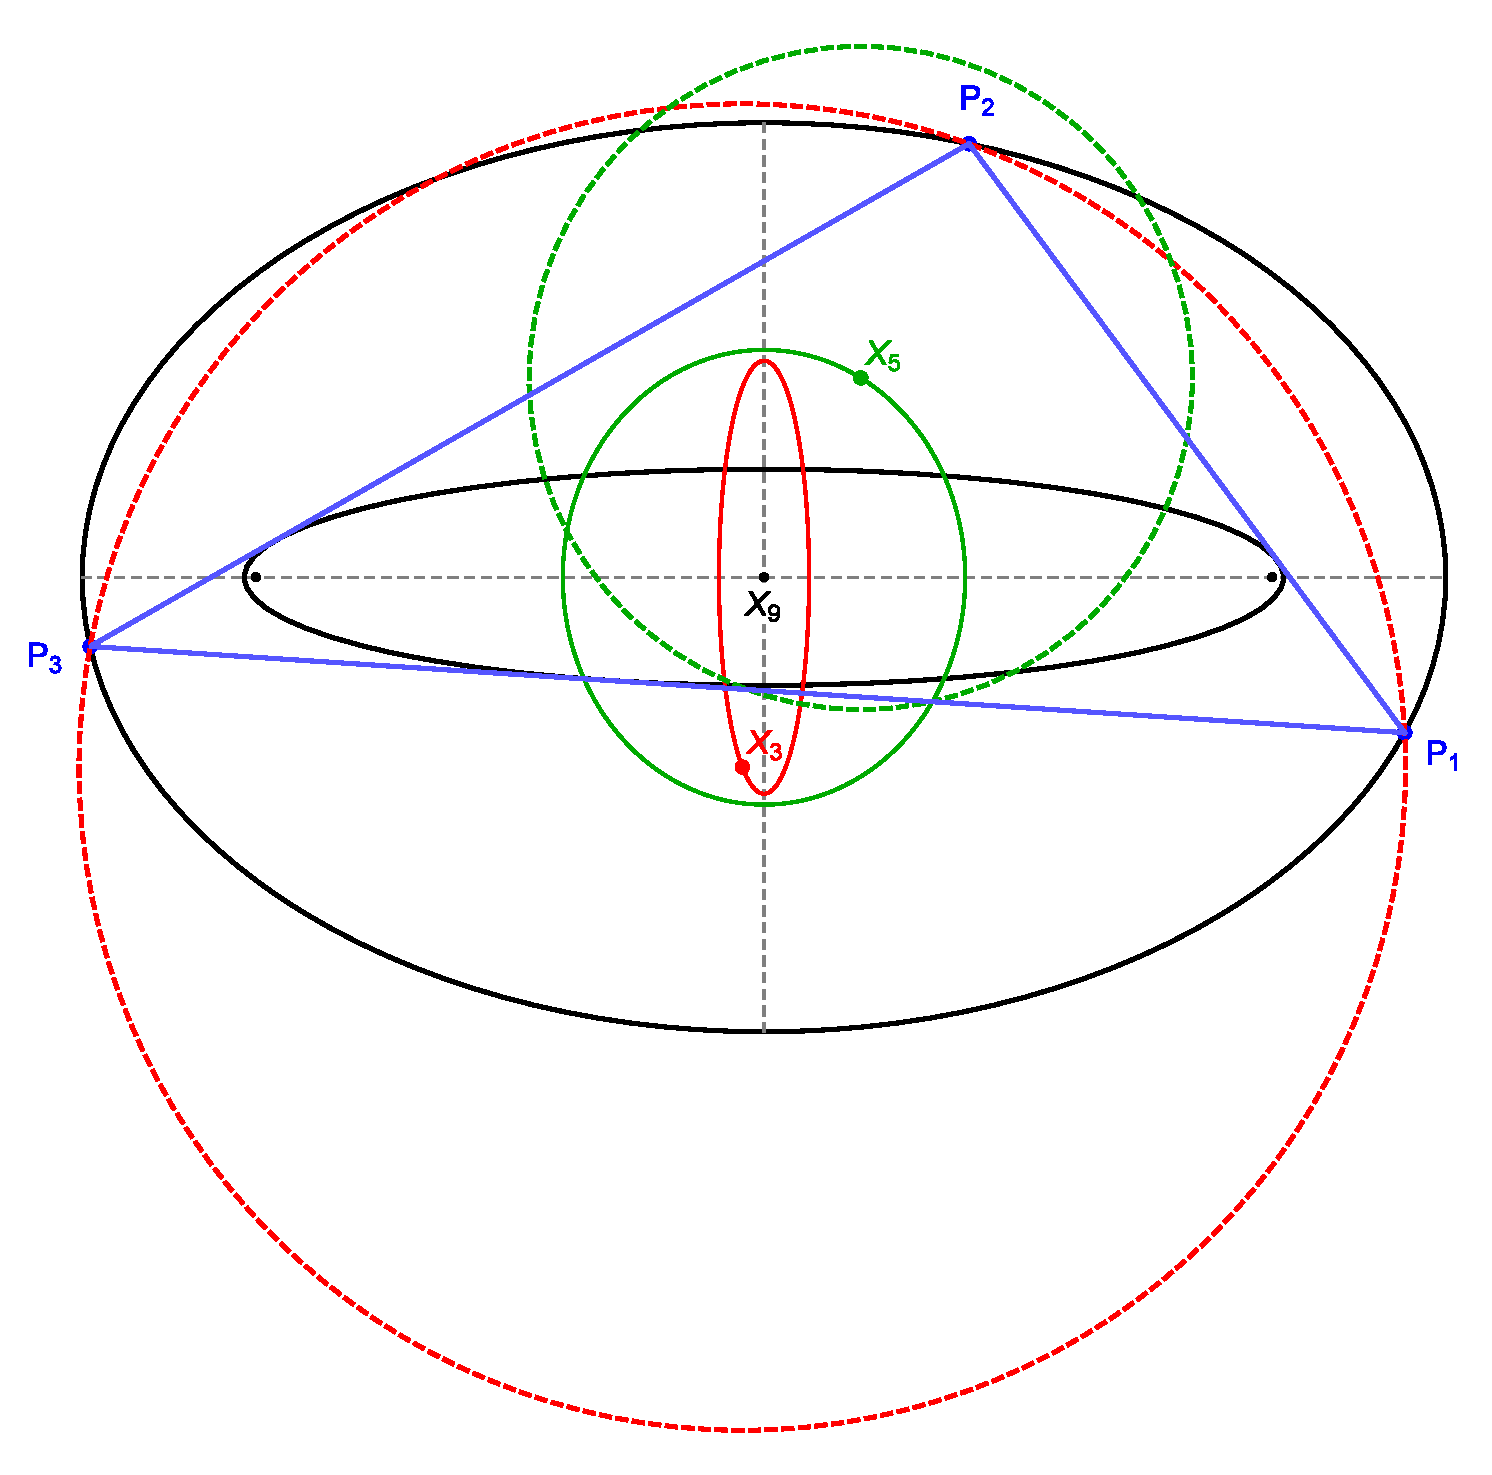
\includegraphics[width=.7\textwidth]{pics/0050_n3_confocal.eps}
    \caption{In the confocal pair (elliptic billiard), the locus of both $X_3$ and $X_5$ are concentric ellipses, (red and green), axis aligned with the original ones. The power of the center $O=X_9$ wrt to either the circumcircle (dashed red) or Euler's circle (dashed green) is invariant. \href{https://bit.ly/3w151N5}{live}}
    \label{fig:confocal}
\end{figure}

\subsection{Excentral to Confocals}

Referring to Figure~\ref{fig:excentral}, the excentral family comprises the excentral triangles to 3-periodics in the elliptic billiard. Abusing notation, here we let $a,b$ denote the axes of said elliptic billiard (i.e., the caustic to the excentral family), and $a_e,b_e$ denote the axes of outer ellipse $\E$, which in \cite{garcia2019-incenter} was derived as:

\begin{equation}
a_e = (a^2+\delta)/b, \;\;\;b_e = (b^2+\delta)/a
\label{eqn:excentrals}
\end{equation}

\noindent where $\delta$ is as in \eqref{eqn:confocal-axes}. Since the Euler's circle of an excentral triangle is the circumcircle of the reference:

\begin{observation}
Over the excentral family $\P_5=-\delta$.
\end{observation}

Still referring to Figure~\ref{fig:excentral}:

\begin{proposition}
In the family of excentral triangles to the confocal family, $\P_3$ is invariant and given by:

\[ \P_3 = -a^2-b^2-2\delta \]
\end{proposition}

\begin{proof}

In the billiard family, straightforward computation of power of $O=X_9$ with respect to Bevan circle (circumcircle of excentral triangle) gives:

\[ \P_3 = \frac{ -12 (s_1 s_2 s_3)^2 }{ (s_1^2 + s_2^2 + s_3^2 - 2 s_1 s_2 - 2 s_2 s_3 - 2 s_3 s_1)^2 }\]

or

\[ \P_3 = \frac{ -48 s^2 }{ (9 - h^2)^2 } =  -a^2-b^2-2\delta \]

\end{proof}

\begin{figure}
    \centering
    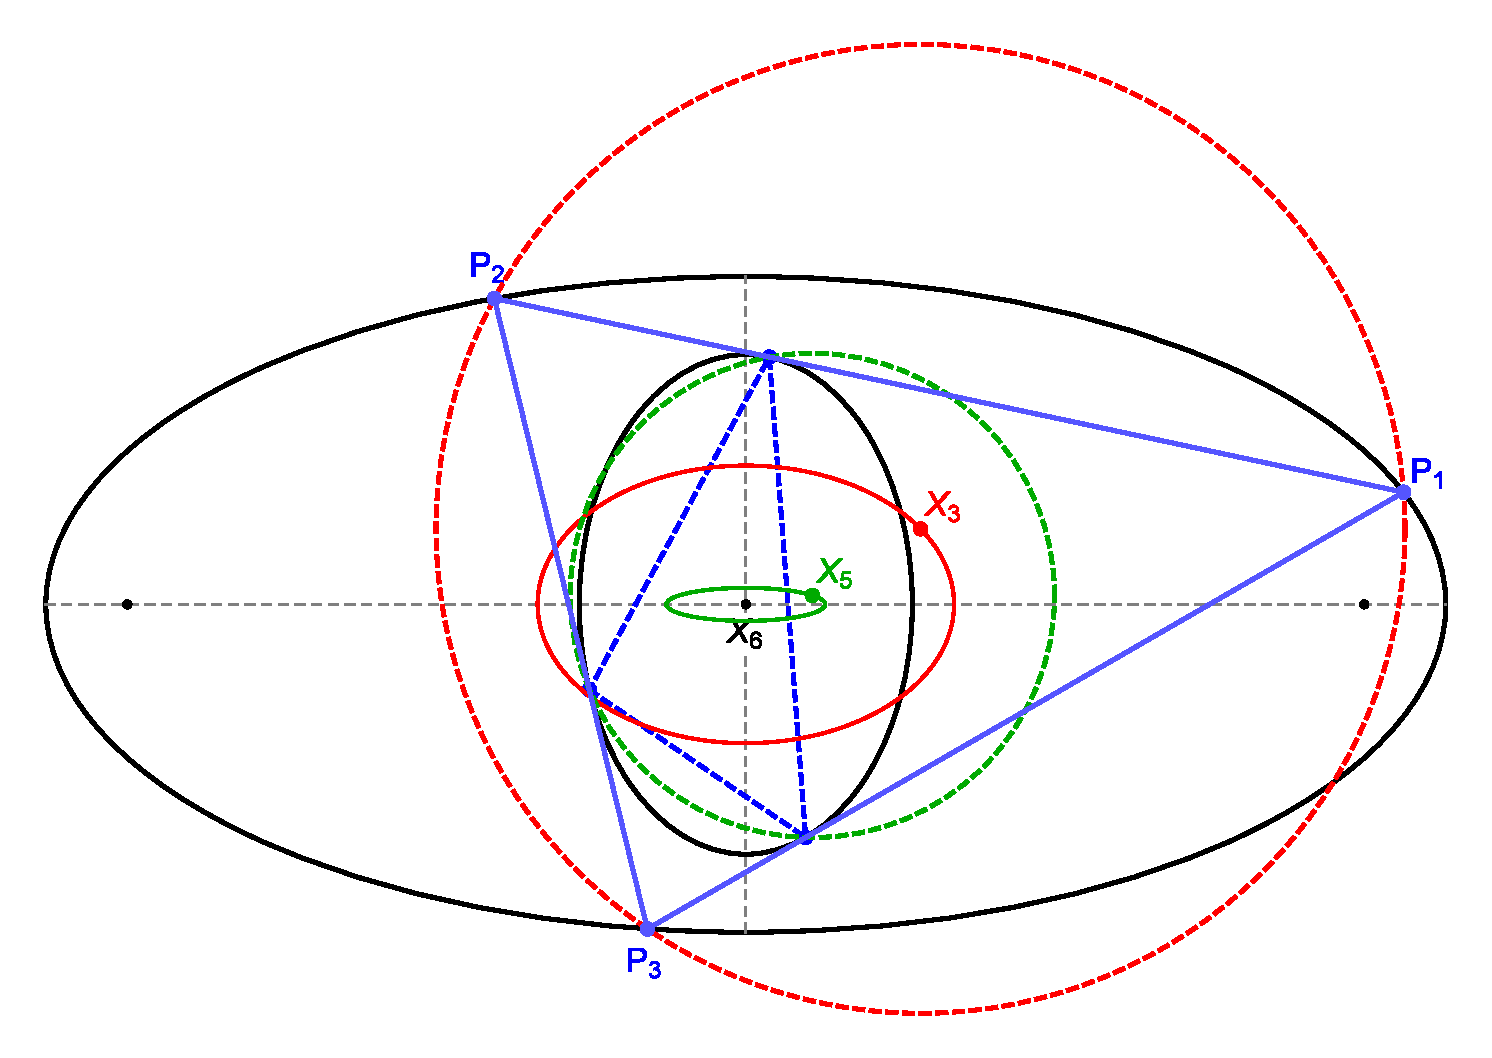
\includegraphics[width=.8\textwidth]{pics/0135_n3_excentral.eps}
    \caption{The excentral family (solid blue) has an elliptic billiard as its caustic, and billiard 3-periodics (dashed blue) as orthic triangles. The power of the symmedian point $X_6$, stationary at the center, with respect to circumcircle (dashed red) and Euler circle (dashed green) is invariant. Also shown are the elliptic loci of their centers $X_3$ and $X_5$ (solid red, solid green), respectively. \href{https://bit.ly/3tV16iY}{live}}
    \label{fig:excentral}
\end{figure}

Note that $\P_3$ for the excentral family is equivalent to the power of the power of the center with respect to the Bevan circle in the confocal family (circumcircle of excenters \cite[Bevan Circle]{mw}).

\subsection*{Summary}

Table~\ref{tab:concentric-summary} summarizes some results in this section. As it will be seen in the next Section, these are special cases of Theorem~\ref{thm:power-concentric-unaligned}.

\begin{table}
\centering
\begin{tabular}{|r|c|l|c|c|}
\hline
family & $N=3$ Cayley & $\P_3$ & $\P_5$ \\
\hline
incircle & $r=(ab)/(a+b)$ & $-ab$ &  $-a b (a^2 + b^2)/(2(a + b)^2)$  \\
circumc. & $a_c+b_c=R$ & $-R^2$ & $-a_c b_c$ \\
homoth. & $a_c=a/2,b_c=b/2$  & $-({a^2+b^2})/{2}$ & $-({a^2+b^2})/{8}$  \\
confocal & see \eqref{eqn:confocal-axes} & $-\delta$ & ${\delta \mu \eta (\mu^2+\eta^2-2)}/{(\mu^2+\eta^2+1)}$\\
excentral & see \eqref{eqn:excentrals} & $-a^2-b^2-2\delta$ & $-\delta$ \\
\hline
\end{tabular}
\caption{Summary of invariant power of origin wrt to circumcircle and Euler's circle for various concentric, axis-aligned systems. Recall $\mu=a/a_c$ and $\eta=b/b_c$.}
\label{tab:concentric-summary}
\end{table}

%$-3(\delta^2-a^2b^2)/(2\delta-a^2-b^2)$

In Appendix~\ref{app:four-more} we show several additional circle-family combinations over which the power of the center is invariant.
